% Appendix A

\chapter{Supplementary Data for Chapter 4}\label{AppendixA}
\lhead{Appendix A. \emph{Supplementary Data for Chapter 4}}

\section{Datasets}

The epitope datasets used in \cref{Chapter4} are detailed below. Each table gives the epitope, MHC class I allele and source protein of the epitope.

\clearpage

\begin{table}[htp]
\begin{center}
\begin{sideways}
{
\scriptsize
\begin{tabulary}{1.5\textwidth}{|l|l|l|l|l|l|l|l|l|l|l|l|}
\hline
Epitope & Allele & Protein & Start & Epitope & Allele & Protein & Start & Epitope & Allele & Protein & Start\bigstrut \\
\hline
AYSSWMYSY & A1 & EBN3\_EBV & 44 & SVASTITGV & A2 & ADFP\_HUMAN & 129 & NAYEYFTKI & B7 & BAK2\_HUMAN & 106 \bigstrut[t] \\
AIVDKVPSV & A2 & COPG\_HUMAN & 147 & SVFAGVVGV & A2 & CYG3\_HUMAN & 581 & NAYVNINRI & B7 & HAPP\_HUMAN & 363 \\
ALADGVQKV & A2 & APL1\_HUMAN & 160 & TIHDIILEC & A2 & VE6\_HPV16 & 29 & NPVPVGNIY & B7 & GAG\_HV2G1 & 257 \\
ALANGIEEV & A2 & APL3\_HUMAN & 172 & TILLGIFFL & A2 & MSHR\_HUMAN & 244 & NSSKVSQNY & B7 & GAG\_HV1J3 & 123 \\
ALASHLIEA & A2 & EHD2\_HUMAN & 507 & VLEETSVML & A2 & VIE1\_HCMVA & 316 & PPIPVGDIY & B7 & GAG\_HV1MA & 259 \\
ALFGALFLA & A2 & PLTP\_HUMAN & 2 & VMAPRTLVL & A2 & 1A23\_HUMAN & 3 & PPSGKGGNY & B7 & GAG\_HV2CA & 127 \\
ALLNIKVKL & A2 & K1CR\_HUMAN & 364 & WLNEVEFKL & A2 & DMD\_HUMAN & 1281 & SPKLPVSSL & B7 & DRI1\_HUMAN & 372 \\
ALLVLYSFA & A2 & LMP1\_EBV & 51 & YLDNGVVFV & A2 & DDB1\_HUMAN & 316 & SPYQNIKIL & B7 & SPSY\_HUMAN & 145 \\
ALPHAILRL & A2 & ACTB\_HUMAN & 170 & YLVTRHADV & A2 & POLG\_HCVH & 1131 & TSEHSHFSL & B7 & DCE2\_HUMAN & 277 \\
FLALIICNA & A2 & MSHR\_HUMAN & 283 & YVDPVITSI & A2 & MET\_HUMAN & 654 & TVLDVGDAY & B7 & POL\_HV1BR & 274 \\
FLDGNELTL & A2 & CLI1\_HUMAN & 167 & DADKYAVTV & B7 & OM1E\_CHLTR & 367 & VFPTKDVAL & B7 & PP65\_HCMVA & 187 \\
FLDGNEMTL & A2 & CLI4\_HUMAN & 178 & DAEMTTRMV & B7 & PSBA\_HUMAN & 90 & VPSEPGGVL & B7 & PTN6\_HUMAN & 422 \\
FLDPRPLTV & A2 & CP1B\_HUMAN & 190 & DAENAMRYI & B7 & CB20\_HUMAN & 93 & WASRELERF & B7 & GAG\_HV1BR & 35 \\
FLLDKKIGV & A2 & TCPB\_HUMAN & 218 & DALLIIPKV & B7 & TCPW\_HUMAN & 441 & YAFNMKATV & B7 & HS7C\_HUMAN & 545 \\
GLIEKNIEL & A2 & DNM1\_HUMAN & 425 & DALLKFSHI & B7 & BI1\_HUMAN & 11 & ELRRKMMYM & B8 & VIE1\_HCMVA & 199 \\
GLLGTLVQL & A2 & CTNB\_HUMAN & 400 & DALLQMITI & B7 & EF2\_HUMAN & 347 & ELRSRYWAI & B8 & VNUC\_IAPUE & 380 \\
GLYPGLIWL & A2 & IRF6\_HUMAN & 21 & DALRSILTI & B7 & SYM\_HUMAN & 703 & GEIYKRWII & B8 & GAG\_HV1BR & 258 \\
KASEKIFYV & A2 & SSX2\_HUMAN & 41 & DAYVLPKLY & B7 & RS26\_HUMAN & 60 & VMLRWGVLA & B8 & NCAP\_HRSVA & 256 \\
LLFDRPMHV & A2 & ROM\_HUMAN & 268 & DGYEQAARV & B7 & TCPE\_HUMAN & 135 & WVKEKVVAL & B8 & NK4\_HUMAN & 175 \\
LLMGTLGIV & A2 & VE7\_HPV16 & 82 & DPYEVSYRI & B7 & BTG1\_HUMAN & 107 & ARFGLIQSM & B27 & Y174\_HUMAN & 81 \\
LTAGFLIFL & A2 & LMP2\_EBV & 453 & DPYKVYRIV & B7 & IRF4\_HUMAN & 120 & GRFSGLLGR & B27 & IL16\_HUMAN & 180 \\
NLLPKLHIV & A2 & CLI1\_HUMAN & 179 & FAYVQIKTI & B7 & CP51\_HUMAN & 454 & GRNVVLDKS & B27 & CH60\_YEREN & 35 \\
NLTISDVSV & A2 & MUC1\_HUMAN & 1133 & HPDIVIYQY & B7 & POL\_HV1U4 & 329 & IRAAPPPLF & B27 & PRTP\_HUMAN & 2 \\
QLIDKVWQL & A2 & SC14\_HUMAN & 593 & IPQQHTQVL & B7 & CEA5\_HUMAN & 632 & IRAASAITA & B27 & CH60\_YEREN & 420 \\
RLVDDFLLV & A2 & TERT\_HUMAN & 865 & KPAFFAEKL & B7 & ANX1\_HUMAN & 273 & IRGAIILAK & B27 & RS2\_HUMAN & 151 \\
SLFPGKLEV & A2 & FLIH\_HUMAN & 1010 & KPSLPFTSL & B7 & CYRG\_HUMAN & 3 & IRLRPGGKK & B27 & GAG\_HV1BR & 18 \\
SLIGHLQTL & A2 & DUS5\_HUMAN & 337 & LPRSTVINI & B7 & IFM1\_HUMAN & 19 & IRNDEELNK & B27 & H2AC\_HUMAN & 87 \\
SLSEKTVLL & A2 & CD59\_HUMAN & 106 & MPMNVADLI & B7 & IF42\_HUMAN & 399 & IRRGVMLAV & B27 & CH60\_HUMAN & 140 \\
SLWGQPAEA & A2 & CA54\_HUMAN & 18 & MPWFKGWKV & B7 & EF11\_HUMAN & 208 & KRGIDKAVI & B27 & CH60\_YEREN & 117 \\
STAPPVHNV & A2 & MUC1\_HUMAN & 950 & NAACMALNI & B7 & OM1E\_CHLTR & 121 & KRIQEIIEQ & B27 & CH60\_HUMAN & 369 \bigstrut[b] \\
\hline
\end{tabulary}
}
\end{sideways}
\end{center}
\caption[The SYF$^1$ dataset]{The SYF$^1$ dataset.}\label{appendixa/table1}
\end{table}

\begin{table}[htp]
\begin{center}
\begin{sideways}
{
\scriptsize
\begin{tabulary}{1.5\textwidth}{|l|l|l|l|l|l|l|l|}
\hline
Epitope & Allele & Protein & Start & Epitope & Allele & Protein & Start \bigstrut \\
\hline
KRTLKIPAM & B27 & CH60\_HUMAN & 469 & ALNFPGSQK & A3 & PM17\_HUMAN & 87 \bigstrut[t] \\
MRMATPLLM & B27 & HG2A\_HUMAN & 107 & RLGVRATRK & A3 & POLG\_HCV1 & 43 \\
NRIVYLYTK & B27 & RL34\_HUMAN & 27 & GPISGHVLK & A3 & PP65\_HCMVA & 16 \\
QRNLYIAGF & B27 & CDM\_HUMAN & 100 & YTPTISRER & A3 & PSB2\_HUMAN & 147 \\
QRNVNIFKF & B27 & LDHA\_HUMAN & 110 & QAIKGMHIR & A3 & RL17\_HUMAN & 34 \\
QRVNVQPEL & B27 & PGTB\_HUMAN & 321 & SLADIMAKR & A3 & RL24\_HUMAN & 86 \\
TRYQGVNLY & B27 & PAB1\_HUMAN & 289 & DTIEIITDR & A3 & ROA2\_HUMAN & 139 \\
AENLWVTVY & B44 & ENV\_HV1S3 & 30 & ETIGEILKK & A3 & ROK\_HUMAN & 95 \\
AETPDIKLF & B44 & RS5\_HUMAN & 12 & FCVGFTKKR & A3 & RS3A\_HUMAN & 137 \\
NEGLGWAGW & B44 & POLG\_HCVJ6 & 88 & EVVVSGKLR & A3 & RS3\_HUMAN & 135 \\
IALYLQQNW & B58 & LMP1\_EBV & 156 & ETFSGVYKK & A3 & RS7\_HUMAN & 171 \\
ITTKAISRW & B58 & TCPG\_HUMAN & 159 & STIEYVIQR & A3 & S23B\_HUMAN & 115 \\
KTKEVIQEW & B58 & TALI\_HUMAN & 343 & TPAGGGFPR & A3 & TISB\_HUMAN & 43 \\
VSFIEFVGW & B58 & EBN4\_EBV & 279 & AIYKQSQHM & A24 & P53\_HUMAN & 161 \\
AFHHVAREL & B62 & NEF\_HV1BR & 190 & AYSQQTRGL & A24 & POLG\_HCVBK & 1031 \\
GFYPGSIEV & B62 & HB2I\_HUMAN & 150 & EYLQLVFGI & A24 & MAG2\_HUMAN & 156 \\
IKADHVSTY & B62 & HA2Q\_HUMAN & 32 & EYLVSFGVW & A24 & CORA\_HPBVJ & 117 \\
WQYFFPVIF & B62 & MAG3\_HUMAN & 143 & HYTNASDGL & A24 & LCK\_HUMAN & 207 \\
DTAAQITQR & A3 & 1B35\_HUMAN & 161 & KYTSFPWLL & A24 & DPOL\_HPBVJ & 756 \\
TIIDILTKR & A3 & ANX1\_HUMAN & 63 & QFQSIYAKF & A24 & RECO\_HUMAN & 47 \\
TIVNILTNR & A3 & ANX2\_HUMAN & 54 & QYDPVAALF & A24 & PP65\_HCMVA & 341 \\
TIIDIITHR & A3 & ANX6\_HUMAN & 384 & RWPSCQKKF & A24 & WT1\_HUMAN & 417 \\
ATIGTAMYK & A3 & BRL1\_EBV & 134 & TFDYLRSVL & A24 & LCK\_HUMAN & 485 \\
GSPATWTTR & A3 & CA34\_HUMAN & 1436 & TYGEIFEKF & A24 & N4BM\_HUMAN & 107 \\
YVNVNMGLK & A3 & CORA\_HPBV4 & 88 & VYAETKHFL & A24 & TERT\_HUMAN & 324 \\
RFKMFPEVK & A3 & DCE2\_HUMAN & 255 & VYALPLKML & A24 & PP65\_HCMVA & 113 \\
TLYCVHQRI & A3 & GAG\_HV1BR & 83 & VYGFVRACL & A24 & TERT\_HUMAN & 461 \\
IVGLNKIVR & A3 & GAG\_HV1EL & 266 & YYMIGEQKF & A24 & NNMT\_HUMAN & 203 \\
DVFVVGTER & A3 & GTFI\_HUMAN & 53 &  &  &  & \\
SIMKWNRER & A3 & NB6M\_HUMAN & 48 &  &  &  & \bigstrut[b] \\
\hline
\end{tabulary}
}
\end{sideways}
\end{center}
\contcaption{Continued}
\end{table}





\begin{table}[htp]
\begin{center}
\begin{sideways}
{
\scriptsize
\begin{tabulary}{1.5\textwidth}{|l|l|l|l|l|l|l|l|l|l|l|l|}
\hline
Epitope & Allele & Protein & HXB2 & Epitope & Allele & Protein & HXB2 & Epitope & Allele & Protein & HXB2 \bigstrut \\
\hline
RRGWEALKY & A1 & gp160 & 787 & TLNAWVKVV & A2 & p24-p2p7p1 & 19 & RLRPGGKKK & A3 & p17 & 20 \bigstrut[t] \\
WIYHTQGYF & A1 & Nef & 113 & AMQMLKETI & A2 & p24-p2p7p1 & 65 & TVRLIKLLY & A3 & Rev & 15 \\
YFPDWQNYT & A1 & Nef & 120 & AEWDRVHPV & A2 & p24-p2p7p1 & 78 & KLLYQSNPP & A3 & Rev & 20 \\
GSEELRSLY & A1 & p17 & 71 & TLQEQIGWM & A2 & p24-p2p7p1 & 110 & RILGTYLGR & A3 & Rev & 58 \\
QRPLVTIKI & A1 & Protease & 7 & MTNNPPIPV & A2 & p24-p2p7p1 & 118 & ALVEICTEM & A3 & RT & 33 \\
ISERILGTY & A1 & Rev & 55 & RMYSPTSIL & A2 & p24-p2p7p1 & 143 & NTPVFAIKK & A3 & RT & 57 \\
LWVTVYYGV & A2 & gp160 & 34 & YVDRFYKTL & A2 & p24-p2p7p1 & 164 & GIPHPAGLK & A3 & RT & 93 \\
VTVYYGVPV & A2 & gp160 & 36 & VLAEAMSQV & A2 & p24-p2p7p1 & 230 & AIFQSSMTK & A3 & RT & 158 \\
NVWATHACV & A2 & gp160 & 67 & LVGPTPVNI & A2 & Protease & 76 & QIYPGIKVR & A3 & RT & 269 \\
QMHEDIISL & A2 & gp160 & 103 & ALVEICTEM & A2 & RT & 33 & QIIEQLIKK & A3 & RT & 520 \\
KLTPLCVSL & A2 & gp160 & 121 & YTAFTIPSI & A2 & RT & 127 & KVYLAWVPA & A3 & RT & 530 \\
KLTSCNTSV & A2 & gp160 & 192 & VIYQYMDDL & A2 & RT & 179 & TACTNCYCK & A3 & Tat & 20 \\
QRGPGRAFV & A2 & gp160 & 310 & YQYMDDLYV & A2 & RT & 181 & HMYVSGKAR & A3 & Vif & 28 \\
TLKQIASKL & A2 & gp160 & 341 & KIEELRQHL & A2 & RT & 201 & KLTEDRWNK & A3 & Vif & 168 \\
TMGAASMTL & A2 & gp160 & 529 & ILKEPVHGV & A2 & RT & 309 & IQRGPGRAF & A24 & gp160 & 309 \\
AVLSIVNRV & A2 & gp160 & 700 & PLVKLWYQL & A2 & RT & 421 & FYCNSTQLF & A24 & gp160 & 383 \\
RLVNGSLAL & A2 & gp160 & 747 & KLGKAGYVT & A2 & RT & 451 & RYLKDQQLL & A24 & gp160 & 585 \\
RLRDLLLIV & A2 & gp160 & 770 & ALQDSGLEV & A2 & RT & 485 & WYIKLFIMI & A24 & gp160 & 680 \\
LLNATAIAV & A2 & gp160 & 814 & AIIRILQQL & A2 & Vpr & 59 & SYHRLRDLL & A24 & gp160 & 767 \\
RVIEVVQGA & A2 & gp160 & 828 & RILQQLLFI & A2 & Vpr & 62 & HSQRRQDIL & A24 & Nef & 102 \\
RIRQGLERI & A2 & gp160 & 846 & VVAIIIAIV & A2 & Vpu & 13 & RQDILDLWI & A24 & Nef & 106 \\
QVRDQAEHL & A2 & Integrase & 164 & SLWDQSLKP & A3 & gp160 & 110 & GYFPDWQNY & A24 & Nef & 119 \\
LLWKGEGAV & A2 & Integrase & 241 & VSFEPIPIH & A3 & gp160 & 208 & DSRLAFHHV & A24 & Nef & 186 \\
ATNAACAWL & A2 & Nef & 50 & HSFNCGGEF & A3 & gp160 & 374 & AFHHVAREL & A24 & Nef & 190 \\
AAVDLSHFL & A2 & Nef & 83 & AVDLSHFLK & A3 & Nef & 84 & KYKLKHIVW & A24 & p17 & 28 \\
YPLTFGWCY & A2 & Nef & 135 & DLSHFLKEK & A3 & Nef & 86 & EIYKRWIIL & A24 & p24-p2p7p1 & 128 \\
LTFGWCYKL & A2 & Nef & 137 & ILDLWIYHT & A3 & Nef & 109 & DYVDRFYKT & A24 & p24-p2p7p1 & 163 \\
LEWRFDSRL & A2 & Nef & 181 & PLTFGWCYK & A3 & Nef & 136 & VYYDPSKDL & A24 & RT & 317 \\
AFHHVAREL & A2 & Nef & 190 & AFHHVAREL & A3 & Nef & 190 & IYQEPFKNL & A24 & RT & 341 \\
SLYNTVATL & A2 & p17 & 77 & KIRLRPGGK & A3 & p17 & 18 & EVIPMFSAL & A26 & p24-p2p7p1 & 35 \bigstrut[b] \\	
\hline
\end{tabulary}
}
\end{sideways}
\end{center}
\caption[The Lanl$^{179}$ dataset]{The Lanl$^{179}$ dataset.}\label{appendixa/table2}
\end{table}

\begin{table}[htp]
\begin{center}
\begin{sideways}
{
\scriptsize
\begin{tabulary}{1.5\textwidth}{|l|l|l|l|l|l|l|l|l|l|l|l|}
\hline
Epitope & Allele & Protein & HXB2 & Epitope & Allele & Protein & HXB2 & Epitope & Allele & Protein & HXB2 \bigstrut \\
\hline
YVDRFYKTL & A26 & p24-p2p7p1 & 164 & GRAFVTIGK & B27 & gp160 & 314 & IVLPEKDSW & B58 & RT & 244 \bigstrut[t] \\
ETKLGKAGY & A26 & RT & 449 & GRRGWEALK & B27 & gp160 & 786 & ITTESIVIW & B58 & RT & 375 \\
IPRRIRQGL & B7 & gp160 & 843 & KIRLRPGGK & B27 & p17 & 18 & VSGKARGWF & B58 & Vif & 31 \\
LPPVVAKEI & B7 & Integrase & 28 & IRLRPGGKK & B27 & p17 & 19 & AVRHFPRIW & B58 & Vpr & 30 \\
FPVTPQVPL & B7 & Nef & 68 & KRWIILGLN & B27 & p24-p2p7p1 & 131 & SFNCGGEFF & B62 & gp160 & 375 \\
TPQVPLRPM & B7 & Nef & 71 & RWIILGLNK & B27 & p24-p2p7p1 & 132 & RAIEAQQHL & B62 & gp160 & 557 \\
RPMTYKAAV & B7 & Nef & 77 & VRHFPRIWL & B27 & Vpr & 31 & THLEGKVIL & B62 & Integrase & 66 \\
TPGPGVRYP & B7 & Nef & 128 & TPQDLNTML & B39 & p24-p2p7p1 & 48 & IKQEFGIPY & B62 & Integrase & 135 \\
YPLTFGWCY & B7 & Nef & 135 & HPVHAGPIA & B39 & p24-p2p7p1 & 84 & RKAKIIRDY & B62 & Integrase & 263 \\
KIRLRPGGK & B7 & p17 & 18 & LEKHGAITS & B44 & Nef & 37 & RMRRAEPAA & B62 & Nef & 19 \\
SPRTLNAWV & B7 & p24-p2p7p1 & 16 & AAVDLSHFL & B44 & Nef & 83 & MTYKAAVDL & B62 & Nef & 79 \\
ATPQDLNTM & B7 & p24-p2p7p1 & 47 & KEKGGLEGL & B44 & Nef & 92 & AAVDLSHFL & B62 & Nef & 83 \\
TPQDLNTML & B7 & p24-p2p7p1 & 48 & GELDRWEKI & B44 & p17 & 11 & YFPDWQNYT & B62 & Nef & 120 \\
HPVHAGPIA & B7 & p24-p2p7p1 & 84 & SEGATPQDL & B44 & p24-p2p7p1 & 44 & LTFGWCYKL & B62 & Nef & 137 \\
ANPDCKTIL & B7 & p24-p2p7p1 & 194 & KETINEEAA & B44 & p24-p2p7p1 & 70 & WRFDSRLAF & B62 & Nef & 183 \\
GPGHKARVL & B7 & p24-p2p7p1 & 223 & EEAAEWDRV & B44 & p24-p2p7p1 & 75 & RLRPGGKKK & B62 & p17 & 20 \\
YPLTSLRSL & B7 & p24-p2p7p1 & 352 & AEWDRVHPV & B44 & p24-p2p7p1 & 78 & RFAVNPGLL & B62 & p17 & 43 \\
SPAIFQSSM & B7 & RT & 156 & CTERQANFL & B44 & p24-p2p7p1 & 294 & VKVVEEKAF & B62 & p24-p2p7p1 & 24 \\
IPLTEEAEL & B7 & RT & 293 & KELYPLTSL & B44 & p24-p2p7p1 & 349 & FSPEVIPMF & B62 & p24-p2p7p1 & 32 \\
YLAWVPAHK & B7 & RT & 532 & IEELRQHLL & B44 & RT & 202 & GHQAAMQML & B62 & p24-p2p7p1 & 61 \\
FPRIWLHGL & B7 & Vpr & 34 & REPHNEWTL & B44 & Vpr & 12 & GLNKIVRMY & B62 & p24-p2p7p1 & 137 \\
RVKEKYQHL & B8 & gp160 & 2 & RAIEAQQHL & B58 & gp160 & 557 & YVDRFYKTL & B62 & p24-p2p7p1 & 164 \\
FNCGGEFFY & B8 & gp160 & 376 & KTAVQMAVF & B58 & Integrase & 173 & GHKAIGTVL & B62 & Protease & 68 \\
GGKKKYKLK & B8 & p17 & 24 & KAAVDLSHF & B58 & Nef & 82 & IHSISERIL & B62 & Rev & 52 \\
ELRSLYNTV & B8 & p17 & 74 & HTQGYFPDW & B58 & Nef & 116 & IPLTEEAEL & B62 & RT & 293 \\
EIKDTKEAL & B8 & p17 & 93 & YTPGPGVRY & B58 & Nef & 127 & DVKQLTEAV & B62 & RT & 364 \\
GEIYKRWII & B8 & p24-p2p7p1 & 127 & ISPRTLNAW & B58 & p24-p2p7p1 & 15 & ITKALGISY & B62 & Tat & 39 \\
NANPDCKTI & B8 & p24-p2p7p1 & 193 & FSPEVIPMF & B58 & p24-p2p7p1 & 32 & WHLGQGVSI & B62 & Vif & 79 \\
DCKTILKAL & B8 & p24-p2p7p1 & 197 & STLQEQIGW & B58 & p24-p2p7p1 & 109 & AVRHFPRIW & B62 & Vpr & 30 \\
GPKVKQWPL & B8 & RT & 18 & QASQEVKNW & B58 & p24-p2p7p1 & 176 & & & & \bigstrut[b] \\		
\hline
\end{tabulary}
}
\end{sideways}
\end{center}
\contcaption{Continued}
\end{table}

\begin{table}[htp]
\begin{center}
\begin{sideways}
{
\tiny
\begin{tabulary}{1.5\textwidth}{|l|l|l|l|l|l|l|l|l|l|l|l|}
\hline
Epitope & Allele & Protein & HXB2 & Epitope & Allele & Protein & HXB2 & Epitope & Allele & Protein & HXB2 \bigstrut \\
\hline
RRGWEALKY & A0101 & gp160 & 787 & KLTSCNTSV & A0202 & gp160 & 192 & LLWKGEGAV & A0203 & Integrase & 241 \bigstrut[t] \\
WIYHTQGYF & A0101 & Nef & 113 & QRGPGRAFV & A0202 & gp160 & 310 & ATNAACAWL & A0203 & Nef & 50 \\
YFPDWQNYT & A0101 & Nef & 120 & TLKQIASKL & A0202 & gp160 & 341 & AAVDLSHFL & A0203 & Nef & 83 \\
GSEELRSLY & A0101 & p17 & 71 & TMGAASMTL & A0202 & gp160 & 529 & YPLTFGWCY & A0203 & Nef & 135 \\
QRPLVTIKI & A0101 & Protease & 7 & AVLSIVNRV & A0202 & gp160 & 700 & LTFGWCYKL & A0203 & Nef & 137 \\
ISERILGTY & A0101 & Rev & 55 & RLVNGSLAL & A0202 & gp160 & 747 & LEWRFDSRL & A0203 & Nef & 181 \\
LWVTVYYGV & A0201 & gp160 & 34 & RLRDLLLIV & A0202 & gp160 & 770 & AFHHVAREL & A0203 & Nef & 190 \\
VTVYYGVPV & A0201 & gp160 & 36 & LLNATAIAV & A0202 & gp160 & 814 & SLYNTVATL & A0203 & p17 & 77 \\
NVWATHACV & A0201 & gp160 & 67 & RVIEVVQGA & A0202 & gp160 & 828 & TLNAWVKVV & A0203 & p24-p2p7p1 & 19 \\
QMHEDIISL & A0201 & gp160 & 103 & RIRQGLERI & A0202 & gp160 & 846 & AMQMLKETI & A0203 & p24-p2p7p1 & 65 \\
KLTPLCVSL & A0201 & gp160 & 121 & QVRDQAEHL & A0202 & Integrase & 164 & AEWDRVHPV & A0203 & p24-p2p7p1 & 78 \\
KLTSCNTSV & A0201 & gp160 & 192 & LLWKGEGAV & A0202 & Integrase & 241 & TLQEQIGWM & A0203 & p24-p2p7p1 & 110 \\
QRGPGRAFV & A0201 & gp160 & 310 & ATNAACAWL & A0202 & Nef & 50 & MTNNPPIPV & A0203 & p24-p2p7p1 & 118 \\
TLKQIASKL & A0201 & gp160 & 341 & AAVDLSHFL & A0202 & Nef & 83 & RMYSPTSIL & A0203 & p24-p2p7p1 & 143 \\
TMGAASMTL & A0201 & gp160 & 529 & YPLTFGWCY & A0202 & Nef & 135 & YVDRFYKTL & A0203 & p24-p2p7p1 & 164 \\
AVLSIVNRV & A0201 & gp160 & 700 & LTFGWCYKL & A0202 & Nef & 137 & VLAEAMSQV & A0203 & p24-p2p7p1 & 230 \\
RLVNGSLAL & A0201 & gp160 & 747 & LEWRFDSRL & A0202 & Nef & 181 & LVGPTPVNI & A0203 & Protease & 76 \\
RLRDLLLIV & A0201 & gp160 & 770 & AFHHVAREL & A0202 & Nef & 190 & ALVEICTEM & A0203 & RT & 33 \\
LLNATAIAV & A0201 & gp160 & 814 & SLYNTVATL & A0202 & p17 & 77 & YTAFTIPSI & A0203 & RT & 127 \\
RVIEVVQGA & A0201 & gp160 & 828 & TLNAWVKVV & A0202 & p24-p2p7p1 & 19 & VIYQYMDDL & A0203 & RT & 179 \\
RIRQGLERI & A0201 & gp160 & 846 & AMQMLKETI & A0202 & p24-p2p7p1 & 65 & YQYMDDLYV & A0203 & RT & 181 \\
QVRDQAEHL & A0201 & Integrase & 164 & AEWDRVHPV & A0202 & p24-p2p7p1 & 78 & KIEELRQHL & A0203 & RT & 201 \\
LLWKGEGAV & A0201 & Integrase & 241 & TLQEQIGWM & A0202 & p24-p2p7p1 & 110 & ILKEPVHGV & A0203 & RT & 309 \\
ATNAACAWL & A0201 & Nef & 50 & MTNNPPIPV & A0202 & p24-p2p7p1 & 118 & PLVKLWYQL & A0203 & RT & 421 \\
AAVDLSHFL & A0201 & Nef & 83 & RMYSPTSIL & A0202 & p24-p2p7p1 & 143 & KLGKAGYVT & A0203 & RT & 451 \\
YPLTFGWCY & A0201 & Nef & 135 & YVDRFYKTL & A0202 & p24-p2p7p1 & 164 & ALQDSGLEV & A0203 & RT & 485 \\
LTFGWCYKL & A0201 & Nef & 137 & VLAEAMSQV & A0202 & p24-p2p7p1 & 230 & AIIRILQQL & A0203 & Vpr & 59 \\
LEWRFDSRL & A0201 & Nef & 181 & LVGPTPVNI & A0202 & Protease & 76 & RILQQLLFI & A0203 & Vpr & 62 \\
AFHHVAREL & A0201 & Nef & 190 & ALVEICTEM & A0202 & RT & 33 & VVAIIIAIV & A0203 & Vpu & 13 \\
SLYNTVATL & A0201 & p17 & 77 & YTAFTIPSI & A0202 & RT & 127 & LWVTVYYGV & A0206 & gp160 & 34 \\
TLNAWVKVV & A0201 & p24-p2p7p1 & 19 & VIYQYMDDL & A0202 & RT & 179 & VTVYYGVPV & A0206 & gp160 & 36 \\
AMQMLKETI & A0201 & p24-p2p7p1 & 65 & YQYMDDLYV & A0202 & RT & 181 & NVWATHACV & A0206 & gp160 & 67 \\
AEWDRVHPV & A0201 & p24-p2p7p1 & 78 & KIEELRQHL & A0202 & RT & 201 & QMHEDIISL & A0206 & gp160 & 103 \\
TLQEQIGWM & A0201 & p24-p2p7p1 & 110 & ILKEPVHGV & A0202 & RT & 309 & KLTPLCVSL & A0206 & gp160 & 121 \\
MTNNPPIPV & A0201 & p24-p2p7p1 & 118 & PLVKLWYQL & A0202 & RT & 421 & KLTSCNTSV & A0206 & gp160 & 192 \\
RMYSPTSIL & A0201 & p24-p2p7p1 & 143 & KLGKAGYVT & A0202 & RT & 451 & QRGPGRAFV & A0206 & gp160 & 310 \\
YVDRFYKTL & A0201 & p24-p2p7p1 & 164 & ALQDSGLEV & A0202 & RT & 485 & TLKQIASKL & A0206 & gp160 & 341 \\
VLAEAMSQV & A0201 & p24-p2p7p1 & 230 & AIIRILQQL & A0202 & Vpr & 59 & TMGAASMTL & A0206 & gp160 & 529 \\
LVGPTPVNI & A0201 & Protease & 76 & RILQQLLFI & A0202 & Vpr & 62 & AVLSIVNRV & A0206 & gp160 & 700 \\
ALVEICTEM & A0201 & RT & 33 & VVAIIIAIV & A0202 & Vpu & 13 & RLVNGSLAL & A0206 & gp160 & 747 \\
YTAFTIPSI & A0201 & RT & 127 & LWVTVYYGV & A0203 & gp160 & 34 & RLRDLLLIV & A0206 & gp160 & 770 \\
VIYQYMDDL & A0201 & RT & 179 & VTVYYGVPV & A0203 & gp160 & 36 & LLNATAIAV & A0206 & gp160 & 814 \\
YQYMDDLYV & A0201 & RT & 181 & NVWATHACV & A0203 & gp160 & 67 & RVIEVVQGA & A0206 & gp160 & 828 \\
KIEELRQHL & A0201 & RT & 201 & QMHEDIISL & A0203 & gp160 & 103 & RIRQGLERI & A0206 & gp160 & 846 \\
ILKEPVHGV & A0201 & RT & 309 & KLTPLCVSL & A0203 & gp160 & 121 & QVRDQAEHL & A0206 & Integrase & 164 \\
PLVKLWYQL & A0201 & RT & 421 & KLTSCNTSV & A0203 & gp160 & 192 & LLWKGEGAV & A0206 & Integrase & 241 \\
KLGKAGYVT & A0201 & RT & 451 & QRGPGRAFV & A0203 & gp160 & 310 & ATNAACAWL & A0206 & Nef & 50 \\
ALQDSGLEV & A0201 & RT & 485 & TLKQIASKL & A0203 & gp160 & 341 & AAVDLSHFL & A0206 & Nef & 83 \\
AIIRILQQL & A0201 & Vpr & 59 & TMGAASMTL & A0203 & gp160 & 529 & YPLTFGWCY & A0206 & Nef & 135 \\
RILQQLLFI & A0201 & Vpr & 62 & AVLSIVNRV & A0203 & gp160 & 700 & LTFGWCYKL & A0206 & Nef & 137 \\
VVAIIIAIV & A0201 & Vpu & 13 & RLVNGSLAL & A0203 & gp160 & 747 & LEWRFDSRL & A0206 & Nef & 181 \\
LWVTVYYGV & A0202 & gp160 & 34 & RLRDLLLIV & A0203 & gp160 & 770 & AFHHVAREL & A0206 & Nef & 190 \\
VTVYYGVPV & A0202 & gp160 & 36 & LLNATAIAV & A0203 & gp160 & 814 & SLYNTVATL & A0206 & p17 & 77 \\
NVWATHACV & A0202 & gp160 & 67 & RVIEVVQGA & A0203 & gp160 & 828 & TLNAWVKVV & A0206 & p24-p2p7p1 & 19 \\
QMHEDIISL & A0202 & gp160 & 103 & RIRQGLERI & A0203 & gp160 & 846 & AMQMLKETI & A0206 & p24-p2p7p1 & 65 \\
KLTPLCVSL & A0202 & gp160 & 121 & QVRDQAEHL & A0203 & Integrase & 164 & AEWDRVHPV & A0206 & p24-p2p7p1 & 78 \bigstrut[b] \\
\hline
\end{tabulary}
}
\end{sideways}
\end{center}
\caption[The Lanl$^{661}$ dataset]{The Lanl$^{661}$ dataset.}\label{appendixa/table3}
\end{table}

\begin{table}[htp]
\begin{center}
\begin{sideways}
{
\tiny
\begin{tabulary}{1.5\textwidth}{|l|l|l|l|l|l|l|l|l|l|l|l|}
\hline
Epitope & Allele & Protein & HXB2 & Epitope & Allele & Protein & HXB2 & Epitope & Allele & Protein & HXB2 \bigstrut \\
\hline
TLQEQIGWM & A0206 & p24-p2p7p1 & 110 & ILKEPVHGV & A0211 & RT & 309 & KLTPLCVSL & A0216 & gp160 & 121 \bigstrut[t] \\
MTNNPPIPV & A0206 & p24-p2p7p1 & 118 & PLVKLWYQL & A0211 & RT & 421 & KLTSCNTSV & A0216 & gp160 & 192 \\
RMYSPTSIL & A0206 & p24-p2p7p1 & 143 & KLGKAGYVT & A0211 & RT & 451 & QRGPGRAFV & A0216 & gp160 & 310 \\
YVDRFYKTL & A0206 & p24-p2p7p1 & 164 & ALQDSGLEV & A0211 & RT & 485 & TLKQIASKL & A0216 & gp160 & 341 \\
VLAEAMSQV & A0206 & p24-p2p7p1 & 230 & AIIRILQQL & A0211 & Vpr & 59 & TMGAASMTL & A0216 & gp160 & 529 \\
LVGPTPVNI & A0206 & Protease & 76 & RILQQLLFI & A0211 & Vpr & 62 & AVLSIVNRV & A0216 & gp160 & 700 \\
ALVEICTEM & A0206 & RT & 33 & VVAIIIAIV & A0211 & Vpu & 13 & RLVNGSLAL & A0216 & gp160 & 747 \\
YTAFTIPSI & A0206 & RT & 127 & LWVTVYYGV & A0212 & gp160 & 34 & RLRDLLLIV & A0216 & gp160 & 770 \\
VIYQYMDDL & A0206 & RT & 179 & VTVYYGVPV & A0212 & gp160 & 36 & LLNATAIAV & A0216 & gp160 & 814 \\
YQYMDDLYV & A0206 & RT & 181 & NVWATHACV & A0212 & gp160 & 67 & RVIEVVQGA & A0216 & gp160 & 828 \\
KIEELRQHL & A0206 & RT & 201 & QMHEDIISL & A0212 & gp160 & 103 & RIRQGLERI & A0216 & gp160 & 846 \\
ILKEPVHGV & A0206 & RT & 309 & KLTPLCVSL & A0212 & gp160 & 121 & QVRDQAEHL & A0216 & Integrase & 164 \\
PLVKLWYQL & A0206 & RT & 421 & KLTSCNTSV & A0212 & gp160 & 192 & LLWKGEGAV & A0216 & Integrase & 241 \\
KLGKAGYVT & A0206 & RT & 451 & QRGPGRAFV & A0212 & gp160 & 310 & ATNAACAWL & A0216 & Nef & 50 \\
ALQDSGLEV & A0206 & RT & 485 & TLKQIASKL & A0212 & gp160 & 341 & AAVDLSHFL & A0216 & Nef & 83 \\
AIIRILQQL & A0206 & Vpr & 59 & TMGAASMTL & A0212 & gp160 & 529 & YPLTFGWCY & A0216 & Nef & 135 \\
RILQQLLFI & A0206 & Vpr & 62 & AVLSIVNRV & A0212 & gp160 & 700 & LTFGWCYKL & A0216 & Nef & 137 \\
VVAIIIAIV & A0206 & Vpu & 13 & RLVNGSLAL & A0212 & gp160 & 747 & LEWRFDSRL & A0216 & Nef & 181 \\
LWVTVYYGV & A0211 & gp160 & 34 & RLRDLLLIV & A0212 & gp160 & 770 & AFHHVAREL & A0216 & Nef & 190 \\
VTVYYGVPV & A0211 & gp160 & 36 & LLNATAIAV & A0212 & gp160 & 814 & SLYNTVATL & A0216 & p17 & 77 \\
NVWATHACV & A0211 & gp160 & 67 & RVIEVVQGA & A0212 & gp160 & 828 & TLNAWVKVV & A0216 & p24-p2p7p1 & 19 \\
QMHEDIISL & A0211 & gp160 & 103 & RIRQGLERI & A0212 & gp160 & 846 & AMQMLKETI & A0216 & p24-p2p7p1 & 65 \\
KLTPLCVSL & A0211 & gp160 & 121 & QVRDQAEHL & A0212 & Integrase & 164 & AEWDRVHPV & A0216 & p24-p2p7p1 & 78 \\
KLTSCNTSV & A0211 & gp160 & 192 & LLWKGEGAV & A0212 & Integrase & 241 & TLQEQIGWM & A0216 & p24-p2p7p1 & 110 \\
QRGPGRAFV & A0211 & gp160 & 310 & ATNAACAWL & A0212 & Nef & 50 & MTNNPPIPV & A0216 & p24-p2p7p1 & 118 \\
TLKQIASKL & A0211 & gp160 & 341 & AAVDLSHFL & A0212 & Nef & 83 & RMYSPTSIL & A0216 & p24-p2p7p1 & 143 \\
TMGAASMTL & A0211 & gp160 & 529 & YPLTFGWCY & A0212 & Nef & 135 & YVDRFYKTL & A0216 & p24-p2p7p1 & 164 \\
AVLSIVNRV & A0211 & gp160 & 700 & LTFGWCYKL & A0212 & Nef & 137 & VLAEAMSQV & A0216 & p24-p2p7p1 & 230 \\
RLVNGSLAL & A0211 & gp160 & 747 & LEWRFDSRL & A0212 & Nef & 181 & LVGPTPVNI & A0216 & Protease & 76 \\
RLRDLLLIV & A0211 & gp160 & 770 & AFHHVAREL & A0212 & Nef & 190 & ALVEICTEM & A0216 & RT & 33 \\
LLNATAIAV & A0211 & gp160 & 814 & SLYNTVATL & A0212 & p17 & 77 & YTAFTIPSI & A0216 & RT & 127 \\
RVIEVVQGA & A0211 & gp160 & 828 & TLNAWVKVV & A0212 & p24-p2p7p1 & 19 & VIYQYMDDL & A0216 & RT & 179 \\
RIRQGLERI & A0211 & gp160 & 846 & AMQMLKETI & A0212 & p24-p2p7p1 & 65 & YQYMDDLYV & A0216 & RT & 181 \\
QVRDQAEHL & A0211 & Integrase & 164 & AEWDRVHPV & A0212 & p24-p2p7p1 & 78 & KIEELRQHL & A0216 & RT & 201 \\
LLWKGEGAV & A0211 & Integrase & 241 & TLQEQIGWM & A0212 & p24-p2p7p1 & 110 & ILKEPVHGV & A0216 & RT & 309 \\
ATNAACAWL & A0211 & Nef & 50 & MTNNPPIPV & A0212 & p24-p2p7p1 & 118 & PLVKLWYQL & A0216 & RT & 421 \\
AAVDLSHFL & A0211 & Nef & 83 & RMYSPTSIL & A0212 & p24-p2p7p1 & 143 & KLGKAGYVT & A0216 & RT & 451 \\
YPLTFGWCY & A0211 & Nef & 135 & YVDRFYKTL & A0212 & p24-p2p7p1 & 164 & ALQDSGLEV & A0216 & RT & 485 \\
LTFGWCYKL & A0211 & Nef & 137 & VLAEAMSQV & A0212 & p24-p2p7p1 & 230 & AIIRILQQL & A0216 & Vpr & 59 \\
LEWRFDSRL & A0211 & Nef & 181 & LVGPTPVNI & A0212 & Protease & 76 & RILQQLLFI & A0216 & Vpr & 62 \\
AFHHVAREL & A0211 & Nef & 190 & ALVEICTEM & A0212 & RT & 33 & VVAIIIAIV & A0216 & Vpu & 13 \\
SLYNTVATL & A0211 & p17 & 77 & YTAFTIPSI & A0212 & RT & 127 & LWVTVYYGV & A0219 & gp160 & 34 \\
TLNAWVKVV & A0211 & p24-p2p7p1 & 19 & VIYQYMDDL & A0212 & RT & 179 & VTVYYGVPV & A0219 & gp160 & 36 \\
AMQMLKETI & A0211 & p24-p2p7p1 & 65 & YQYMDDLYV & A0212 & RT & 181 & NVWATHACV & A0219 & gp160 & 67 \\
AEWDRVHPV & A0211 & p24-p2p7p1 & 78 & KIEELRQHL & A0212 & RT & 201 & QMHEDIISL & A0219 & gp160 & 103 \\
TLQEQIGWM & A0211 & p24-p2p7p1 & 110 & ILKEPVHGV & A0212 & RT & 309 & KLTPLCVSL & A0219 & gp160 & 121 \\
MTNNPPIPV & A0211 & p24-p2p7p1 & 118 & PLVKLWYQL & A0212 & RT & 421 & KLTSCNTSV & A0219 & gp160 & 192 \\
RMYSPTSIL & A0211 & p24-p2p7p1 & 143 & KLGKAGYVT & A0212 & RT & 451 & QRGPGRAFV & A0219 & gp160 & 310 \\
YVDRFYKTL & A0211 & p24-p2p7p1 & 164 & ALQDSGLEV & A0212 & RT & 485 & TLKQIASKL & A0219 & gp160 & 341 \\
VLAEAMSQV & A0211 & p24-p2p7p1 & 230 & AIIRILQQL & A0212 & Vpr & 59 & TMGAASMTL & A0219 & gp160 & 529 \\
LVGPTPVNI & A0211 & Protease & 76 & RILQQLLFI & A0212 & Vpr & 62 & AVLSIVNRV & A0219 & gp160 & 700 \\
ALVEICTEM & A0211 & RT & 33 & VVAIIIAIV & A0212 & Vpu & 13 & RLVNGSLAL & A0219 & gp160 & 747 \\
YTAFTIPSI & A0211 & RT & 127 & LWVTVYYGV & A0216 & gp160 & 34 & RLRDLLLIV & A0219 & gp160 & 770 \\
VIYQYMDDL & A0211 & RT & 179 & VTVYYGVPV & A0216 & gp160 & 36 & LLNATAIAV & A0219 & gp160 & 814 \\
YQYMDDLYV & A0211 & RT & 181 & NVWATHACV & A0216 & gp160 & 67 & RVIEVVQGA & A0219 & gp160 & 828 \\
KIEELRQHL & A0211 & RT & 201 & QMHEDIISL & A0216 & gp160 & 103 & RIRQGLERI & A0219 & gp160 & 846 \bigstrut[b] \\
\hline
\end{tabulary}
}
\end{sideways}
\end{center}
\contcaption{Continued}
\end{table}

\begin{table}[htp]
\begin{center}
\begin{sideways}
{
\tiny
\begin{tabulary}{1.5\textwidth}{|l|l|l|l|l|l|l|l|l|l|l|l|}
\hline
Epitope & Allele & Protein & HXB2 & Epitope & Allele & Protein & HXB2 & Epitope & Allele & Protein & HXB2 \bigstrut \\
\hline
QVRDQAEHL & A0219 & Integrase & 164 & DLSHFLKEK & A1101 & Nef & 86 & RLRPGGKKK & A3001 & p17 & 20 \bigstrut[t] \\
LLWKGEGAV & A0219 & Integrase & 241 & TLYCVHQRI & A1101 & p17 & 84 & KQNPDIVIY & A3001 & RT & 173 \\
ATNAACAWL & A0219 & Nef & 50 & AIFQSSMTK & A1101 & RT & 158 & KLNWASQIY & A3001 & RT & 263 \\
AAVDLSHFL & A0219 & Nef & 83 & QIYPGIKVR & A1101 & RT & 269 & QRGPGRAFV & A3002 & gp160 & 310 \\
YPLTFGWCY & A0219 & Nef & 135 & FVNTPPLVK & A1101 & RT & 416 & IVNRVRQGY & A3002 & gp160 & 704 \\
LTFGWCYKL & A0219 & Nef & 137 & QIIEQLIKK & A1101 & RT & 520 & KYWWNLLQY & A3002 & gp160 & 794 \\
LEWRFDSRL & A0219 & Nef & 181 & RYLKDQQLL & A2301 & gp160 & 585 & KIQNFRVYY & A3002 & Integrase & 219 \\
AFHHVAREL & A0219 & Nef & 190 & KYKLKHIVW & A2301 & p17 & 28 & RLRPGGKKK & A3002 & p17 & 20 \\
SLYNTVATL & A0219 & p17 & 77 & IYQEPFKNL & A2301 & RT & 341 & KQNPDIVIY & A3002 & RT & 173 \\
TLNAWVKVV & A0219 & p24-p2p7p1 & 19 & IQRGPGRAF & A2402 & gp160 & 309 & KLNWASQIY & A3002 & RT & 263 \\
AMQMLKETI & A0219 & p24-p2p7p1 & 65 & FYCNSTQLF & A2402 & gp160 & 383 & VRYPLTFGW & A3301 & Nef & 133 \\
AEWDRVHPV & A0219 & p24-p2p7p1 & 78 & RYLKDQQLL & A2402 & gp160 & 585 & RLAFHHVAR & A3301 & Nef & 188 \\
TLQEQIGWM & A0219 & p24-p2p7p1 & 110 & WYIKLFIMI & A2402 & gp160 & 680 & MVHQAISPR & A3301 & p24-p2p7p1 & 10 \\
MTNNPPIPV & A0219 & p24-p2p7p1 & 118 & SYHRLRDLL & A2402 & gp160 & 767 & AIFQSSMTK & A3301 & RT & 158 \\
RMYSPTSIL & A0219 & p24-p2p7p1 & 143 & HSQRRQDIL & A2402 & Nef & 102 & FYVDGAANR & A3301 & RT & 440 \\
YVDRFYKTL & A0219 & p24-p2p7p1 & 164 & RQDILDLWI & A2402 & Nef & 106 & EYRKILRQR & A3301 & Vpu & 29 \\
VLAEAMSQV & A0219 & p24-p2p7p1 & 230 & GYFPDWQNY & A2402 & Nef & 119 & ETAYFLLKL & A6801 & Integrase & 96 \\
LVGPTPVNI & A0219 & Protease & 76 & DSRLAFHHV & A2402 & Nef & 186 & VTLWQRPLV & A6801 & Protease & 3 \\
ALVEICTEM & A0219 & RT & 33 & AFHHVAREL & A2402 & Nef & 190 & DTVLEEMSL & A6801 & Protease & 30 \\
YTAFTIPSI & A0219 & RT & 127 & KYKLKHIVW & A2402 & p17 & 28 & NTPVFAIKK & A6801 & RT & 57 \\
VIYQYMDDL & A0219 & RT & 179 & EIYKRWIIL & A2402 & p24-p2p7p1 & 128 & AIFQSSMTK & A6801 & RT & 158 \\
YQYMDDLYV & A0219 & RT & 181 & DYVDRFYKT & A2402 & p24-p2p7p1 & 163 & ETAYFLLKL & A6802 & Integrase & 96 \\
KIEELRQHL & A0219 & RT & 201 & VYYDPSKDL & A2402 & RT & 317 & VTLWQRPLV & A6802 & Protease & 3 \\
ILKEPVHGV & A0219 & RT & 309 & IYQEPFKNL & A2402 & RT & 341 & DTVLEEMSL & A6802 & Protease & 30 \\
PLVKLWYQL & A0219 & RT & 421 & IQRGPGRAF & A2403 & gp160 & 309 & NTPVFAIKK & A6802 & RT & 57 \\
KLGKAGYVT & A0219 & RT & 451 & FYCNSTQLF & A2403 & gp160 & 383 & AIFQSSMTK & A6802 & RT & 158 \\
ALQDSGLEV & A0219 & RT & 485 & RYLKDQQLL & A2403 & gp160 & 585 & RAEPAADRV & A6901 & Nef & 22 \\
AIIRILQQL & A0219 & Vpr & 59 & WYIKLFIMI & A2403 & gp160 & 680 & RVGAASRDL & A6901 & Nef & 29 \\
RILQQLLFI & A0219 & Vpr & 62 & SYHRLRDLL & A2403 & gp160 & 767 & IPRRIRQGL & B0702 & gp160 & 843 \\
VVAIIIAIV & A0219 & Vpu & 13 & HSQRRQDIL & A2403 & Nef & 102 & LPPVVAKEI & B0702 & Integrase & 28 \\
SLWDQSLKP & A0301 & gp160 & 110 & RQDILDLWI & A2403 & Nef & 106 & FPVTPQVPL & B0702 & Nef & 68 \\
VSFEPIPIH & A0301 & gp160 & 208 & GYFPDWQNY & A2403 & Nef & 119 & TPQVPLRPM & B0702 & Nef & 71 \\
HSFNCGGEF & A0301 & gp160 & 374 & DSRLAFHHV & A2403 & Nef & 186 & RPMTYKAAV & B0702 & Nef & 77 \\
AVDLSHFLK & A0301 & Nef & 84 & AFHHVAREL & A2403 & Nef & 190 & TPGPGVRYP & B0702 & Nef & 128 \\
DLSHFLKEK & A0301 & Nef & 86 & KYKLKHIVW & A2403 & p17 & 28 & YPLTFGWCY & B0702 & Nef & 135 \\
ILDLWIYHT & A0301 & Nef & 109 & EIYKRWIIL & A2403 & p24-p2p7p1 & 128 & KIRLRPGGK & B0702 & p17 & 18 \\
PLTFGWCYK & A0301 & Nef & 136 & DYVDRFYKT & A2403 & p24-p2p7p1 & 163 & SPRTLNAWV & B0702 & p24-p2p7p1 & 16 \\
AFHHVAREL & A0301 & Nef & 190 & VYYDPSKDL & A2403 & RT & 317 & ATPQDLNTM & B0702 & p24-p2p7p1 & 47 \\
KIRLRPGGK & A0301 & p17 & 18 & IYQEPFKNL & A2403 & RT & 341 & TPQDLNTML & B0702 & p24-p2p7p1 & 48 \\
RLRPGGKKK & A0301 & p17 & 20 & EVIPMFSAL & A2601 & p24-p2p7p1 & 35 & HPVHAGPIA & B0702 & p24-p2p7p1 & 84 \\
TVRLIKLLY & A0301 & Rev & 15 & YVDRFYKTL & A2601 & p24-p2p7p1 & 164 & ANPDCKTIL & B0702 & p24-p2p7p1 & 194 \\
KLLYQSNPP & A0301 & Rev & 20 & ETKLGKAGY & A2601 & RT & 449 & GPGHKARVL & B0702 & p24-p2p7p1 & 223 \\
RILGTYLGR & A0301 & Rev & 58 & EVIPMFSAL & A2602 & p24-p2p7p1 & 35 & YPLTSLRSL & B0702 & p24-p2p7p1 & 352 \\
ALVEICTEM & A0301 & RT & 33 & YVDRFYKTL & A2602 & p24-p2p7p1 & 164 & SPAIFQSSM & B0702 & RT & 156 \\
NTPVFAIKK & A0301 & RT & 57 & ETKLGKAGY & A2602 & RT & 449 & IPLTEEAEL & B0702 & RT & 293 \\
GIPHPAGLK & A0301 & RT & 93 & SFEPIPIHY & A2902 & gp160 & 209 & YLAWVPAHK & B0702 & RT & 532 \\
AIFQSSMTK & A0301 & RT & 158 & FNCGGEFFY & A2902 & gp160 & 376 & FPRIWLHGL & B0702 & Vpr & 34 \\
QIYPGIKVR & A0301 & RT & 269 & RIKQIINMW & A2902 & gp160 & 419 & RVKEKYQHL & B0801 & gp160 & 2 \\
QIIEQLIKK & A0301 & RT & 520 & YFPDWQNYT & A2902 & Nef & 120 & FNCGGEFFY & B0801 & gp160 & 376 \\
KVYLAWVPA & A0301 & RT & 530 & LYNTVATLY & A2902 & p17 & 78 & GGKKKYKLK & B0801 & p17 & 24 \\
TACTNCYCK & A0301 & Tat & 20 & NCYCKKCCF & A2902 & Tat & 24 & ELRSLYNTV & B0801 & p17 & 74 \\
HMYVSGKAR & A0301 & Vif & 28 & HIVSPRCEY & A2902 & Vif & 127 & EIKDTKEAL & B0801 & p17 & 93 \\
KLTEDRWNK & A0301 & Vif & 168 & QRGPGRAFV & A3001 & gp160 & 310 & GEIYKRWII & B0801 & p24-p2p7p1 & 127 \\
SVITQACPK & A1101 & gp160 & 199 & IVNRVRQGY & A3001 & gp160 & 704 & NANPDCKTI & B0801 & p24-p2p7p1 & 193 \\
NTLKQIASK & A1101 & gp160 & 340 & KYWWNLLQY & A3001 & gp160 & 794 & DCKTILKAL & B0801 & p24-p2p7p1 & 197 \\
AVDLSHFLK & A1101 & Nef & 84 & KIQNFRVYY & A3001 & Integrase & 219 & GPKVKQWPL & B0801 & RT & 18 \bigstrut[b] \\
\hline
\end{tabulary}
}
\end{sideways}
\end{center}
\contcaption{Continued}
\end{table}

\begin{table}[htp]
\begin{center}
\begin{sideways}
{
\tiny
\begin{tabulary}{1.5\textwidth}{|l|l|l|l|l|l|l|l|l|l|l|l|}
\hline
Epitope & Allele & Protein & HXB2 & Epitope & Allele & Protein & HXB2 & Epitope & Allele & Protein & HXB2 \bigstrut \\
\hline
RVKEKYQHL & B0802 & gp160 & 2 & TVLDVGDAY & B3501 & RT & 107 & DSRLAFHHV & B5101 & Nef & 186 \bigstrut[t] \\
FNCGGEFFY & B0802 & gp160 & 376 & FSVPLDEDF & B3501 & RT & 116 & AFHHVAREL & B5101 & Nef & 190 \\
GGKKKYKLK & B0802 & p17 & 24 & SPAIFQSSM & B3501 & RT & 156 & NANPDCKTI & B5101 & p24-p2p7p1 & 193 \\
ELRSLYNTV & B0802 & p17 & 74 & NPDIVIYQY & B3501 & RT & 175 & EKEGKISKI & B5101 & RT & 42 \\
EIKDTKEAL & B0802 & p17 & 93 & IPLTEEAEL & B3501 & RT & 293 & QGWKGSPAI & B5101 & RT & 151 \\
GEIYKRWII & B0802 & p24-p2p7p1 & 127 & EPIVGAETF & B3501 & RT & 432 & IPLTEEAEL & B5101 & RT & 293 \\
NANPDCKTI & B0802 & p24-p2p7p1 & 193 & DARLVITTY & B3501 & Vif & 61 & EPIVGAETF & B5101 & RT & 432 \\
DCKTILKAL & B0802 & p24-p2p7p1 & 197 & HTGERDWHL & B3501 & Vif & 73 & EAVRHFPRI & B5101 & Vpr & 29 \\
GPKVKQWPL & B0802 & RT & 18 & TPQDLNTML & B3901 & p24-p2p7p1 & 48 & YPLTFGWCY & B5301 & Nef & 135 \\
SFNCGGEFF & B1501 & gp160 & 375 & HPVHAGPIA & B3901 & p24-p2p7p1 & 84 & TPQDLNTML & B5301 & p24-p2p7p1 & 48 \\
RAIEAQQHL & B1501 & gp160 & 557 & LEKHGAITS & B4001 & Nef & 37 & PPIPVGEIY & B5301 & p24-p2p7p1 & 122 \\
THLEGKVIL & B1501 & Integrase & 66 & AAVDLSHFL & B4001 & Nef & 83 & QASQEVKNW & B5301 & p24-p2p7p1 & 176 \\
IKQEFGIPY & B1501 & Integrase & 135 & KEKGGLEGL & B4001 & Nef & 92 & ASQEVKNWM & B5301 & p24-p2p7p1 & 177 \\
RKAKIIRDY & B1501 & Integrase & 263 & GELDRWEKI & B4001 & p17 & 11 & TPPQKQEPI & B5301 & p24-p2p7p1 & 339 \\
RMRRAEPAA & B1501 & Nef & 19 & SEGATPQDL & B4001 & p24-p2p7p1 & 44 & YPLTSLRSL & B5301 & p24-p2p7p1 & 352 \\
MTYKAAVDL & B1501 & Nef & 79 & KETINEEAA & B4001 & p24-p2p7p1 & 70 & IPLTEEAEL & B5301 & RT & 293 \\
AAVDLSHFL & B1501 & Nef & 83 & EEAAEWDRV & B4001 & p24-p2p7p1 & 75 & RAIEAQQHL & B5701 & gp160 & 557 \\
YFPDWQNYT & B1501 & Nef & 120 & AEWDRVHPV & B4001 & p24-p2p7p1 & 78 & KTAVQMAVF & B5701 & Integrase & 173 \\
LTFGWCYKL & B1501 & Nef & 137 & CTERQANFL & B4001 & p24-p2p7p1 & 294 & KAAVDLSHF & B5701 & Nef & 82 \\
WRFDSRLAF & B1501 & Nef & 183 & KELYPLTSL & B4001 & p24-p2p7p1 & 349 & HTQGYFPDW & B5701 & Nef & 116 \\
RLRPGGKKK & B1501 & p17 & 20 & IEELRQHLL & B4001 & RT & 202 & YFPDWQNYT & B5701 & Nef & 120 \\
RFAVNPGLL & B1501 & p17 & 43 & REPHNEWTL & B4001 & Vpr & 12 & YTPGPGVRY & B5701 & Nef & 127 \\
VKVVEEKAF & B1501 & p24-p2p7p1 & 24 & LEKHGAITS & B4002 & Nef & 37 & LTFGWCYKL & B5701 & Nef & 137 \\
FSPEVIPMF & B1501 & p24-p2p7p1 & 32 & AAVDLSHFL & B4002 & Nef & 83 & ISPRTLNAW & B5701 & p24-p2p7p1 & 15 \\
GHQAAMQML & B1501 & p24-p2p7p1 & 61 & KEKGGLEGL & B4002 & Nef & 92 & FSPEVIPMF & B5701 & p24-p2p7p1 & 32 \\
GLNKIVRMY & B1501 & p24-p2p7p1 & 137 & GELDRWEKI & B4002 & p17 & 11 & STLQEQIGW & B5701 & p24-p2p7p1 & 109 \\
YVDRFYKTL & B1501 & p24-p2p7p1 & 164 & SEGATPQDL & B4002 & p24-p2p7p1 & 44 & QASQEVKNW & B5701 & p24-p2p7p1 & 176 \\
GHKAIGTVL & B1501 & Protease & 68 & KETINEEAA & B4002 & p24-p2p7p1 & 70 & FSVPLDEDF & B5701 & RT & 116 \\
IHSISERIL & B1501 & Rev & 52 & EEAAEWDRV & B4002 & p24-p2p7p1 & 75 & IVLPEKDSW & B5701 & RT & 244 \\
IPLTEEAEL & B1501 & RT & 293 & AEWDRVHPV & B4002 & p24-p2p7p1 & 78 & ITTESIVIW & B5701 & RT & 375 \\
DVKQLTEAV & B1501 & RT & 364 & CTERQANFL & B4002 & p24-p2p7p1 & 294 & VSGKARGWF & B5701 & Vif & 31 \\
ITKALGISY & B1501 & Tat & 39 & KELYPLTSL & B4002 & p24-p2p7p1 & 349 & AVRHFPRIW & B5701 & Vpr & 30 \\
WHLGQGVSI & B1501 & Vif & 79 & IEELRQHLL & B4002 & RT & 202 & RAIEAQQHL & B5801 & gp160 & 557 \\
AVRHFPRIW & B1501 & Vpr & 30 & REPHNEWTL & B4002 & Vpr & 12 & KTAVQMAVF & B5801 & Integrase & 173 \\
TEKLWVTVY & B1801 & gp160 & 31 & TEKLWVTVY & B4402 & gp160 & 31 & KAAVDLSHF & B5801 & Nef & 82 \\
YDTEVHNVW & B1801 & gp160 & 61 & LYNTVATLY & B4402 & p17 & 78 & HTQGYFPDW & B5801 & Nef & 116 \\
QDILDLWIY & B1801 & Nef & 107 & EEKAFSPEV & B4402 & p24-p2p7p1 & 28 & YTPGPGVRY & B5801 & Nef & 127 \\
YPLTFGWCY & B1801 & Nef & 135 & SEGATPQDL & B4402 & p24-p2p7p1 & 44 & ISPRTLNAW & B5801 & p24-p2p7p1 & 15 \\
NNETPGIRY & B1801 & RT & 136 & QEPIDKELY & B4402 & p24-p2p7p1 & 344 & FSPEVIPMF & B5801 & p24-p2p7p1 & 32 \\
NPDIVIYQY & B1801 & RT & 175 & EEMSLPGRW & B4402 & Protease & 34 & STLQEQIGW & B5801 & p24-p2p7p1 & 109 \\
GRAFVTIGK & B2705 & gp160 & 314 & EELRQHLLR & B4402 & RT & 203 & QASQEVKNW & B5801 & p24-p2p7p1 & 176 \\
GRRGWEALK & B2705 & gp160 & 786 & TEKLWVTVY & B4403 & gp160 & 31 & IVLPEKDSW & B5801 & RT & 244 \\
KIRLRPGGK & B2705 & p17 & 18 & LYNTVATLY & B4403 & p17 & 78 & ITTESIVIW & B5801 & RT & 375 \\
IRLRPGGKK & B2705 & p17 & 19 & EEKAFSPEV & B4403 & p24-p2p7p1 & 28 & VSGKARGWF & B5801 & Vif & 31 \\
RWIILGLNK & B2705 & p24-p2p7p1 & 132 & SEGATPQDL & B4403 & p24-p2p7p1 & 44 & AVRHFPRIW & B5801 & Vpr & 30 \\
VRHFPRIWL & B2705 & Vpr & 31 & QEPIDKELY & B4403 & p24-p2p7p1 & 344 &  &  &  &  \\
DPNPQEVVL & B3501 & gp160 & 78 & EEMSLPGRW & B4403 & Protease & 34 &  &  &  &  \\
RPVVSTQLL & B3501 & gp160 & 252 & EELRQHLLR & B4403 & RT & 203 &  &  &  &  \\
TAVPWNASW & B3501 & gp160 & 606 & EEKAFSPEV & B4501 & p24-p2p7p1 & 28 &  &  &  &  \\
FPVTPQVPL & B3501 & Nef & 68 & AETFYVDGA & B4501 & RT & 437 &  &  &  &  \\
WIYHTQGYF & B3501 & Nef & 113 & DPNPQEVVL & B5101 & gp160 & 78 &  &  &  &  \\
YPLTFGWCY & B3501 & Nef & 135 & LPCRIKQII & B5101 & gp160 & 416 &  &  &  &  \\
RPGGKKKYK & B3501 & p17 & 22 & RAIEAQQHL & B5101 & gp160 & 557 &  &  &  &  \\
WASRELERF & B3501 & p17 & 36 & GACRAIRHI & B5101 & gp160 & 835 &  &  &  &  \\
HSNQVSQNY & B3501 & p17 & 124 & LPPVVAKEI & B5101 & Integrase & 28 &  &  &  &  \\
PPIPVGEIY & B3501 & p24-p2p7p1 & 122 & YFPDWQNYT & B5101 & Nef & 120 &  &  &  & \bigstrut[b] \\
\hline
\end{tabulary}
}
\end{sideways}
\end{center}
\contcaption{Continued}
\end{table}

\clearpage

\section{The HIV HXB2 Proteome}

The viral strain HXB2 (\tref{appendixa/HXB2}) (GenBank Accession Number \href{http://www.ncbi.nlm.nih.gov/nuccore/1906382}{K03455}) is used as a reference strain for the HIV epitope datasets in \cref{Chapter4}. The position of the defined epitope location relative to the sequence of the HXB2 protein is indicated in these datasets. HXB2 was selected as the reference strain because so many studies use HXB2, and because crystal structures for HXB2-related proteins are available.

\begin{table}[htp]
\begin{center}
\begin{tabulary}{\textwidth}{|L|}
\hline
gp160 \bigstrut[t] \\
MRVKEKYQHLWRWGWRWGTMLLGMLMICSATEKLWVTVYYGVPVWKEATT \bigstrut[t] \\
TLFCASDAKAYDTEVHNVWATHACVPTDPNPQEVVLVNVTENFNMWKNDM \\
VEQMHEDIISLWDQSLKPCVKLTPLCVSLKCTDLKNDTNTNSSSGRMIME \\
KGEIKNCSFNISTSIRGKVQKEYAFFYKLDIIPIDNDTTSYKLTSCNTSV \\
ITQACPKVSFEPIPIHYCAPAGFAILKCNNKTFNGTGPCTNVSTVQCTHG \\
IRPVVSTQLLLNGSLAEEEVVIRSVNFTDNAKTIIVQLNTSVEINCTRPN \\
NNTRKRIRIQRGPGRAFVTIGKIGNMRQAHCNISRAKWNNTLKQIASKLR \\
EQFGNNKTIIFKQSSGGDPEIVTHSFNCGGEFFYCNSTQLFNSTWFNSTW \\
STEGSNNTEGSDTITLPCRIKQIINMWQKVGKAMYAPPISGQIRCSSNIT \\
GLLLTRDGGNSNNESEIFRPGGGDMRDNWRSELYKYKVVKIEPLGVAPTK \\
AKRRVVQREKRAVGIGALFLGFLGAAGSTMGAASMTLTVQARQLLSGIVQ \\
QQNNLLRAIEAQQHLLQLTVWGIKQLQARILAVERYLKDQQLLGIWGCSG \\
KLICTTAVPWNASWSNKSLEQIWNHTTWMEWDREINNYTSLIHSLIEESQ \\
NQQEKNEQELLELDKWASLWNWFNITNWLWYIKLFIMIVGGLVGLRIVFA \\
VLSIVNRVRQGYSPLSFQTHLPTPRGPDRPEGIEEEGGERDRDRSIRLVN \\
GSLALIWDDLRSLCLFSYHRLRDLLLIVTRIVELLGRRGWEALKYWWNLL \\
QYWSQELKNSAVSLLNATAIAVAEGTDRVIEVVQGACRAIRHIPRRIRQG \\
LERILL \bigstrut[b] \\
\hline
Integrase \bigstrut[t] \\
FLDGIDKAQDEHEKYHSNWRAMASDFNLPPVVAKEIVASCDKCQLKGEAM \bigstrut[t] \\
HGQVDCSPGIWQLDCTHLEGKVILVAVHVASGYIEAEVIPAETGQETAYF \\
LLKLAGRWPVKTIHTDNGSNFTGATVRAACWWAGIKQEFGIPYNPQSQGV \\
VESMNKELKKIIGQVRDQAEHLKTAVQMAVFIHNFKRKGGIGGYSAGERI \\
VDIIATDIQTKELQKQITKIQNFRVYYRDSRNPLWKGPAKLLWKGEGAVV \\
IQDNSDIKVVPRRKAKIIRDYGKQMAGDDCVASRQDED \bigstrut[b] \\
\hline
Nef \bigstrut[t] \\
MGGKWSKSSVIGWPTVRERMRRAEPAADRVGAASRDLEKHGAITSSNTAA \bigstrut[t] \\ 
TNAACAWLEAQEEEEVGFPVTPQVPLRPMTYKAAVDLSHFLKEKGGLEGL \\
IHSQRRQDILDLWIYHTQGYFPDWQNYTPGPGVRYPLTFGWCYKLVPVEP \\
DKIEEANKGENTSLLHPVSLHGMDDPEREVLEWRFDSRLAFHHVARELHP \\
EYFKNC \bigstrut[b] \\
\hline
p17 \bigstrut[t] \\
MGARASVLSGGELDRWEKIRLRPGGKKKYKLKHIVWASRELERFAVNPGL \bigstrut[t] \\
LETSEGCRQILGQLQPSLQTGSEELRSLYNTVATLYCVHQRIEIKDTKEA \\
LDKIEEEQNKSKKKAQQAAADTGHSNQVSQNY \bigstrut[b] \\
\hline
p24-p2p7p1p6 \bigstrut[t] \\
PIVQNIQGQMVHQAISPRTLNAWVKVVEEKAFSPEVIPMFSALSEGATPQ \bigstrut[t] \\
DLNTMLNTVGGHQAAMQMLKETINEEAAEWDRVHPVHAGPIAPGQMREPR \\
GSDIAGTTSTLQEQIGWMTNNPPIPVGEIYKRWIILGLNKIVRMYSPTSI \\
LDIRQGPKEPFRDYVDRFYKTLRAEQASQEVKNWMTETLLVQNANPDCKT \\
ILKALGPAATLEEMMTACQGVGGPGHKARVLAEAMSQVTNSATIMMQRGN \\
FRNQRKIVKCFNCGKEGHTARNCRAPRKKGCWKCGKEGHQMKDCTERQAN \\
FLGKIWPSYKGRPGNFLQSRPEPTAPPEESFRSGVETTTPPQKQEPIDKE \\
LYPLTSLRSLFGNDPSSQ \bigstrut[b] \\
\hline
\end{tabulary}
\end{center}
\caption[The HIV HXB2 proteome]{The HIV HXB2 proteome}\label{appendixa/HXB2}
\end{table}


\begin{table}[t]
\begin{center}
\begin{tabulary}{\textwidth}{|L|}
\hline
Protease \bigstrut[t] \\
PQVTLWQRPLVTIKIGGQLKEALLDTGADDTVLEEMSLPGRWKPKMIGGI \bigstrut[t] \\
GGFIKVRQYDQILIEICGHKAIGTVLVGPTPVNIIGRNLLTQIGCTLNF \bigstrut[b] \\
\hline
Rev \bigstrut[t] \\
MAGRSGDSDEELIRTVRLIKLLYQSNPPPNPEGTRQARRNRRRRWRERQR \bigstrut[t] \\
QIHSISERILGTYLGRSAEPVPLQLPPLERLTLDCNEDCGTSGTQGVGSP \\
QILVESPTVLESGTKE \bigstrut[b] \\
\hline
RT \bigstrut[t] \\
PISPIETVPVKLKPGMDGPKVKQWPLTEEKIKALVEICTEMEKEGKISKI \bigstrut[t] \\
GPENPYNTPVFAIKKKDSTKWRKLVDFRELNKRTQDFWEVQLGIPHPAGL \bigstrut[b] \\
\hline
\end{tabulary}
\end{center}
\contcaption{Continued}
\end{table}


\section{The Effect of Set Size on ROC Curves}\label{AppendixA/sizeEffects}

From \sref{chapter4/results/NegVol}, we examined the effect of a reduced negative dataset on rescaling and we found that rescaling still significantly reduced epitope detection accuracy. \fref{chapter4/figureEffectPos} and \fref{chapter4/figureEffectNeg} show a more general examination of the effect on AUC values when the positive and negative set sizes are altered.

We used epitope data from the SYF$^1$ dataset (\sref{chapter4/methodsDatasets}) to test two effects: the change in AUC values when the positive (epitope) set size is changed with a constant negative (random peptide) set size, and vice versa. \fref{chapter4/figureEffectPos} shows that changing the positive set size has no significant effect on the AUC values. However, increasing the negative set size significantly increases the AUC value (\fref{chapter4/figureEffectNeg}, $P < 0.001$). The reason for this is that, assuming the positive set size is drawn from the same distribution, the proportion of epitopes discovered as the threshold changes would not vary even as the positive set size increases. However, increasing the negative set size increases the ratio of true positives to true negatives at any threshold, which would result in a larger AUC value. Although this may be viewed as a trivial result, it is worth bearing in mind when comparing AUC values across different datasets. 


\begin{figure}[htp]
\centering
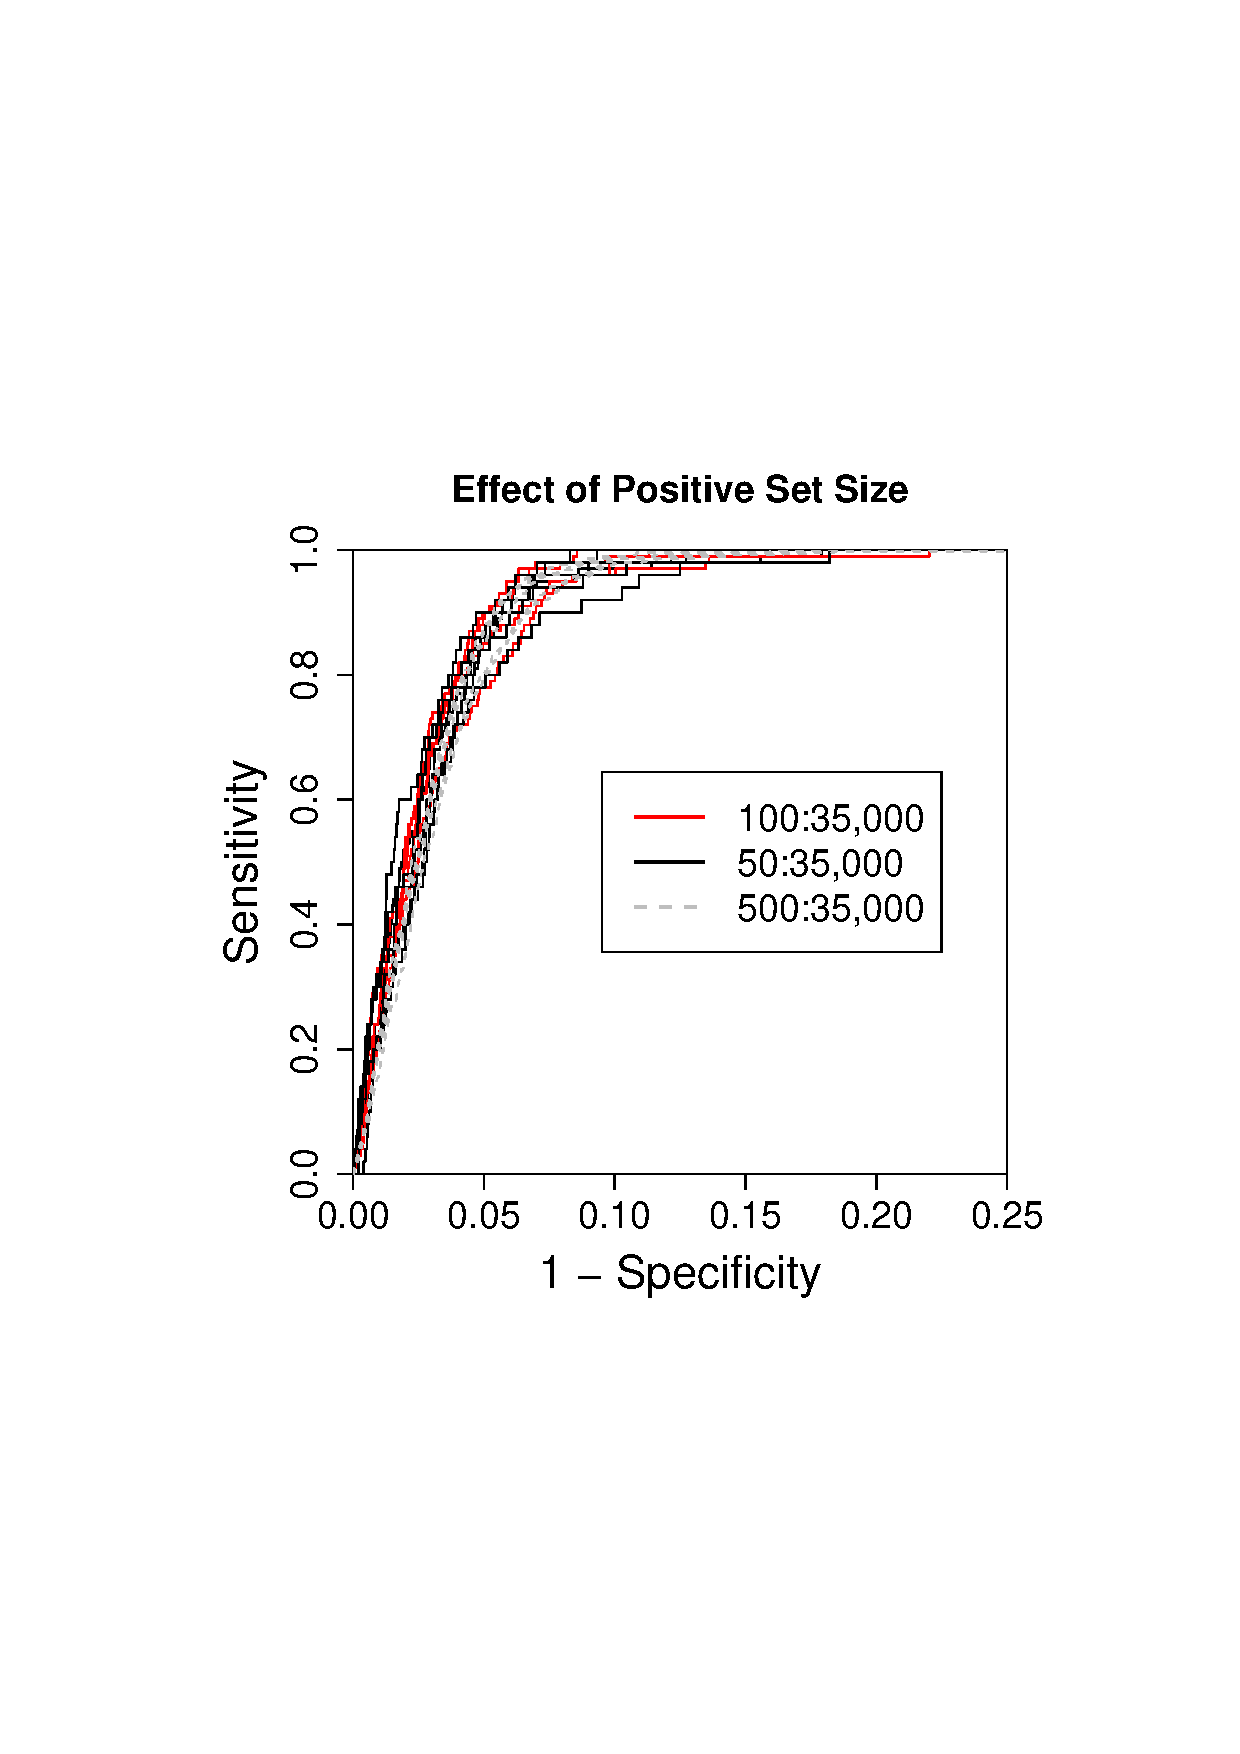
\includegraphics[width=10cm]{./Figures/chapter4/effectSizePositive}
\caption[The effect of positive set size]{The effect of positive set size on AUC values. The data for each ROC curve was randomly assigned from the SYF$^1$ dataset. For each size classification, 5 random samples of positive and negative data was used.}
\label{chapter4/figureEffectPos}
\end{figure}

\begin{figure}[htp]
\centering
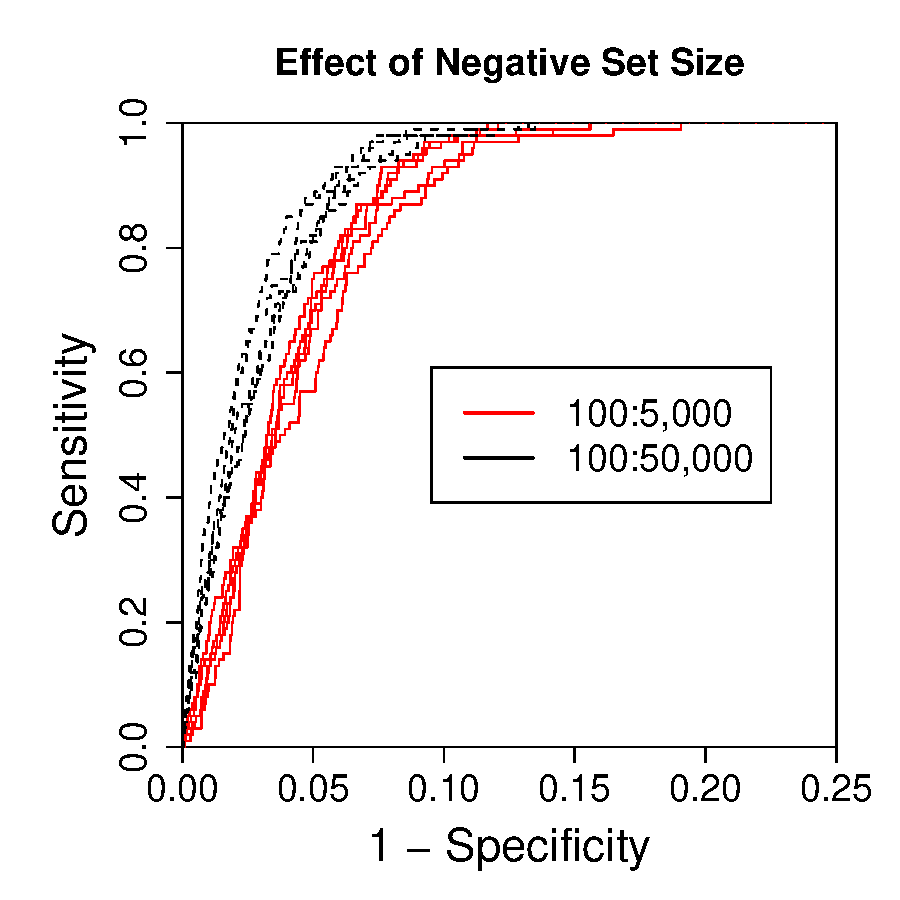
\includegraphics[width=10cm]{./Figures/chapter4/effectSizeNegative}
\caption[The effect of negative set size]{The effect of neagative set size on AUC values. The positive and negative data was selected as in \fref{chapter4/figureEffectPos}.}
\label{chapter4/figureEffectNeg}
\end{figure}

